%----------------------------------------------------------------------------------------
%	Hardware
%----------------------------------------------------------------------------------------

\chapter{Hardware Components}

The hardware must obtain electrical signals corresponding to the amount of weight applied to the scale. Weight sensing occurs via load cells, which are electrical sensors that react to changes in applied weight. The team must develop circuitry to connect the load cells and obtain electrical signals from them. However, load cells change resistance minimally with weight applied. Thus signals obtained from them are small and circuitry is required to amplify and process the signals to be measurable by an ADC. This section details the hardware design, including research on prior solutions, load cells, sensing and processing circuits, and the proposed design.

\section{Prior Art}

In this section, existing hardware solutions for digital weighing scales are evaluated. A digital weighing scale is a common measurement device, thus there are many existing products on the market. Some existing options are detailed and compared below.

The 2nd Gen Xiaomi Smart Scale is an intelligent scale that has the primary function of weighing people, with many extra functions that allow fitness tracking with connected accounts. The technical specifications consist of: High precision pressure sensors that can measure still items over 100g and accurately perceive subtle changes of 50g, Bluetooth 5.0 connectivity for devices to track body information via the Xiaomi sports APP. The dimensions are: 300 x 300 x 20mm. Data such as body balance, weight and BMI uploaded and tracked on the sports app, as well as diet and fitness plans. Home members can be automatically identified when used, with up to 16 members. Many functionalities improve the interactions of the product such as body tracking and small item measurements. However, the higher price does not appeal to people that are not willing to spend much on a scale

The Living \& Co Digital Glass Scale is a cheap alternative of a weight scale with little extra functionality. It is for people that only require the bare minimum out of a weight scale, with a “high precision strain-gauge sensor” that will always give you accuracy every time. The dimensions are: 290 x 280 x 20mm. Real-Time measurements are updated instantly with no extra processing. This scale is made for people without a bigger budget or people not willing to invest in a weight scale. This lack of extra functionality also means that it is easier for people to use, however, it means it is only limited to one function. Bad reviews about massive fluctuations in measurements also sets this product back.

The FItBit Aria Air is a smart scale that functions as a regular weighing scale, but also records weights and synchronises the users biometrics to the FitBit app. The technical specifications consist of: Bluetooth functionality to connect to devices that track body information via the FitBit app, and it has dimensions of 300 x 300 x 20mm. In terms of functionality, the scale syncs the weight to the FitBit app where people can view their trends and see other details recorded by FitBit trackers and watches such as BMI. Users can use their smartphone Bluetooth technology to set up and interact with their scale too. The scale has many functionalities that improve the interactions of the product such as body tracking and small item measurements. FitBit is a very popular health brand that benefits the user if they have more ways to measure health metrics. Unfortunately, this means that the proprietary applications result in limited competition for FitBit users, and the higher price does not appeal to people that are not willing to spend much on a scale

Generally, all physical weight scales are the same, with differences being in the more expensive range having the ability to connect to other devices where weight metrics are processed with other body measurements to give users more information on their health. This principle can be applied to not only humans, but also dogs. Our focus is to provide the weights of dogs, but also to upload that information to a database where further processing may take place, or purely just to track weight.

\section{Load Cell Working Principles}

This section explains the working principles of the load cells. A strain gauge is an electrical sensor that reacts to weight by having an electrical resistance that either increases or decreases when weight is applied. A load cell uses several strain gauges to measure weight more accurately than one strain gauge. The provided load cells consist of two strain gauges as in Figure \ref{fig:load_cell}. One’s resistance decreases linearly with weight, and the other’s resistance increases linearly. To connect the load cells to circuitry, three wires are accessible; one at the midpoint of the resistors and one at each end. Four load cells are provided, with one at each corner of the scale, referred to as R1, R2, R3, and R4.

\begin{figure}[!ht]
	\centering
	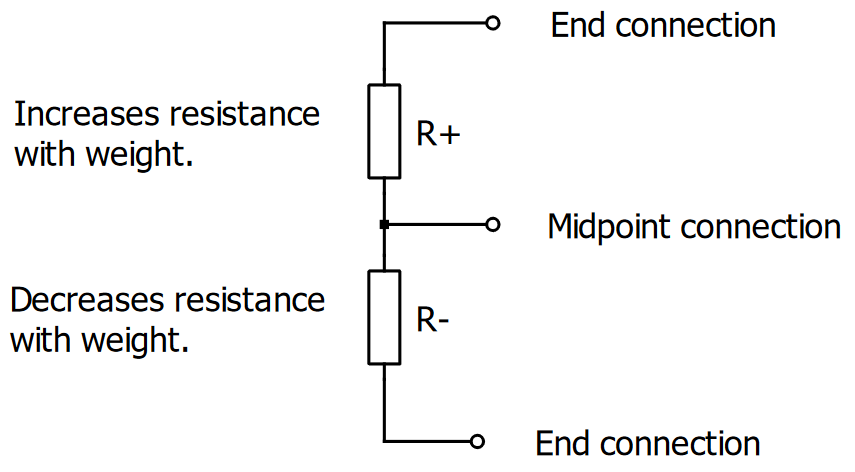
\includegraphics[scale=0.4]{load-cell.png}
	\caption{Diagram of the provided load cell.}
	\label{fig:load_cell}
\end{figure}

\section{Sensing Topologies}
In this section, topologies to connect the load cells are compared.
The load cells could individually be connected to the ADC to gain a measurement from each, as in Figure A.1. This would allow weight distribution to be sensed across the scale by gaining measurements from each corner; however, it requires four signals to be input to the ADC. With only three ADC ports, this option is only possible if an external ADC is used at additional cost. An extra cost is also incurred from requiring four processing circuits.

Another option is connecting all load cells together in a parallel configuration as in Figure A.2 and sending one signal to the ADC. This option is low cost as it only requires one processing circuit. However, parallel connections reduce resolution because each load cell's resistance changes are averaged instead of being added.

Alternatively, each load cell could be connected in a Wheatstone bridge as in Figure A.3.a. This topology is used to detect small changes in resistance and produces a high-resolution output. Having one Wheatstone bridge per load cell would allow the sensing of weight distribution, however, it is unfeasible because of the number of ADC ports. Two load cells could be placed in one Wheatstone bridge for two outputs. This allows weight distribution sensing across halves of the scale, however, this provides little benefit over a single output and incurs additional cost. As such, all four load cells can be connected in one Wheatstone bridge as in Figure A.3.b. Adding multiple load cells in the Wheatstone bridge does not reduce resolution because differences are added and not averaged. Further, this option only requires one processing circuit; thus is a low-cost solution. 


\section{Processing Topologies}
This section discusses requirements for the processing circuit and compares topologies to process the signals from the sensing circuit.

Processing the signal from the sensing circuit is required because the signal is small and the ADC of the Raspberry Pi Pico has requirements and limitations. Further, amplification requires an operational amplifier (op-amp), a common amplification device. However, low-cost op-amps are not able to output tiny signals. Thus, the requirements for the output signal are: the signal should be between 0 V and 3.3V for the ADC, the signal should maximise this range to maximise resolution, and an offset to the signal is required to meet the op-amp requirements.

To produce an offset, a Zener regulator may be used as in Figure A.4.a. However, the offset it produces is limited to standard values and thus is not a flexible solution. Alternatively, resistors may be used to divide the supply voltage down. However, the circuitry it is added to may draw current from it, thus changing the offset value (the loading effect). Therefore, this solution is not reliable. An op-amp buffer may be placed after the voltage divider as in Figure A.4.b to prevent loading because it prevents current from being drawn from the resistors, thus allowing a stable offset.

The signal must also be amplified. An inverting or non-inverting op-amp amplifier may be used. However, these solutions only accept single ended inputs, and the Wheatstone bridge produces a double ended output, thus are not suitable. As such, a differential amplifier as in Figure A.5 would be suitable. However, it is susceptible to the loading effect (as defined earlier). To prevent this, an instrumentation amplifier can be used as in Figure A.6.

In any electrical signal, unwanted high-frequency harmonics or noise is present. Noise in the output signal will reduce the accuracy of the ADC reading. To minimise its effects, a filter should be implemented. A simple resistor capacitor (RC) filter as in Figure A.7 will be used to keep the design simple and cheap. An op-amp (active) filter could be used; however, active filters are complex and unnecessary for a signal that varies slowly with time.


\section{The Proposed Design}
This section outlines the proposed design, including a schematic, simulation results, and specifications. The design comprises a Wheatstone bridge, instrumentation amplifier, and RC filter, as in Figure \ref{fig:schematic}.

\begin{figure}[!ht]
	\centering
	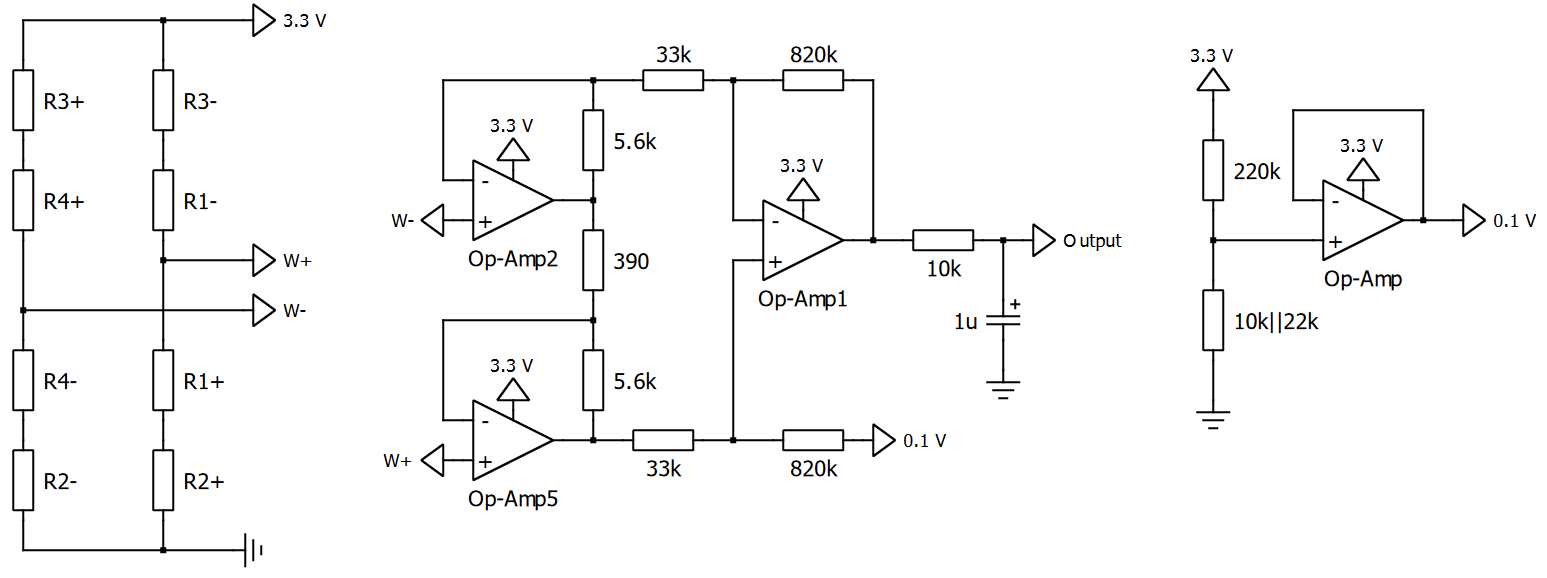
\includegraphics[scale=0.35]{schematic.png}
	\caption{Hardware schematic for signal sensing, processing, and offset generation.}
	\label{fig:schematic}
\end{figure}

The design was simulated using LTSpice as in Figure \ref{fig:simulation}. Values from practical testing were used for base resistance of resistors and the amount of change of resistance as weight is applied. The output varies linearly, and is amplified and offset successfully.

\begin{figure}[!ht]
	\centering
	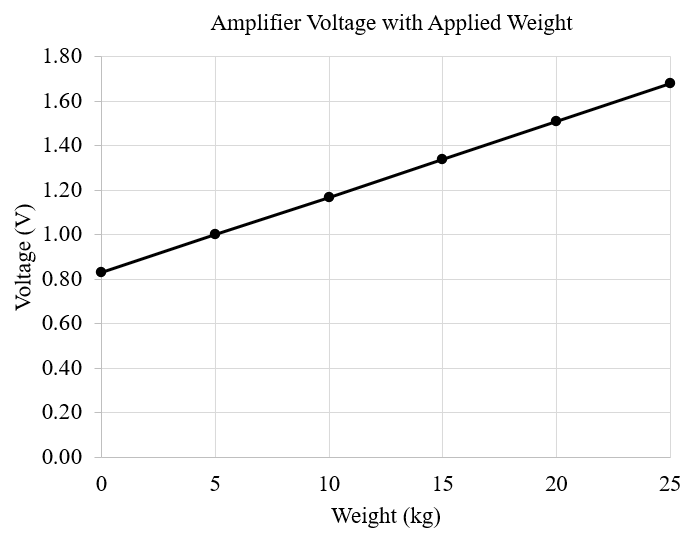
\includegraphics[scale=0.4]{simulation.png}
	\caption{Hardware simulation results of sensing and processing circuits.}
	\label{fig:simulation}
\end{figure}

The gain and offset were chosen based on a cheap op-amp (LM324N), which has a range from 20 mV to 1.8 V. Thus, the gain and offset are 100mV and 714 V/V respectively to maximise this range. The Wheatstone bridge has a 1 mV offset due to differences in base resistance, resulting in a 800 mV offset once amplified.

Functional and technical specifications are outlined below.

Functional specifications:
\begin{itemize}
    \item Operating voltage:	3.3 V
    \item Measurement range:	0 kg to 25 kg
    \item Measurement resolution: 	0.5 kg
    \item Method of zeroing scale:	Button
\end{itemize}

Technical specifications:
\begin{itemize}
    \item Number of load cells:	4
    \item Sensing circuit topology:	Single Wheatstone bridge
    \item Processing circuit topology:	Instrumentation amplifier
    \item Gain of processing circuit:	714 V/V
    \item Offset of processing circuit:	0.1 V
    \item Range of output:               	0.8 V - 1.8 V
\end{itemize}